\scanpage{37}
% archive sheet number: 36
$K\subset\mathbb C$, $\bar K$ algebraic closure in $\mathbb C$, $\pi_1=\pi_1(\mathrm{Spec}\,K,\bar K)=\mathrm{Gal}(\bar K/K)$, $\unsure{A|\mathcal A}={}$ring of ``finite'' adèles of $\mathbb Q$. We \unsure{$^{1}$|$^{l}$}consider a category of motives over $K$, of finite type, and the Galois group \inserted{$G$} associated with the Betti functor. This gives rise to the following structures.

% Diagram across the head of the sheet; the small boxes share their frames' corners.
\diagram{\resizebox{\linewidth}{!}{\begin{tikzcd}[ampersand replacement=\&,column sep=4pt,row sep=7pt,execute at end picture={
 \draw ([xshift=-5pt,yshift=6pt]gd.north west) rectangle ([xshift=5pt,yshift=-8pt]gp.east |- gm.south);
 \node[draw,anchor=south east,inner sep=1pt] at ([xshift=5pt,yshift=-8pt]gp.east |- gm.south) {$D$};
 \draw ([xshift=-5pt,yshift=6pt]p.north west) rectangle ([xshift=5pt,yshift=-12pt]g.south east);
 \node[draw,anchor=south east,inner sep=1pt] at ([xshift=5pt,yshift=-12pt]g.south east) {$B$};
 \draw (p.south) -- (avec.north);
 \draw (conn.center) ellipse [x radius=38pt,y radius=13pt];
 \draw (pc.south) -- (ptc.north);
 \draw (qc.south) -- (ptq.north);
 \draw (ptc.center) ellipse [x radius=37pt,y radius=14pt];
 \node[draw,anchor=south east,inner sep=1pt] at ([xshift=5pt,yshift=-3pt]ptc.south east) {$C$};
 \node[draw,anchor=south east,inner sep=1pt] at (ga.south east) {$A$};
}]
 |[alias=gd]| G''_K \arrow[r,phantom,"{\supset}" description] \& H''_K\arrow[r,dash,dashed] \& Q\arrow[r,dash,dashed] \& H'_K \&[-4pt] {\subset} \&[-4pt] |[alias=gp]| G'_K\arrow[r,dash,dashed] \& |[alias=p]| P\arrow[r,dash,dashed] \& |[alias=g]| G_K \&[13pt] |[alias=pc]| P_{\mathbb C} \& G_{\mathbb C} \& |[alias=qc]| Q_{\mathbb C} \&[8pt] |[draw,alias=ga,minimum width=34pt,minimum height=24pt]| G\\
 |[alias=gm]| \mathbb G_m\arrow[u,shift left=1,"i_1"]\arrow[u,shift right=1,"i_2"'] \& \& \& \& \& \& |[alias=avec]| \text{with} \& \& |[alias=ptc]| \begin{gathered}\text{with point }\deleted{\unsure{\xi|a}}\ \alpha\\\text{rational over }\mathbb C,\ \text{so}\end{gathered} \& \& |[alias=ptq]| \begin{gathered}\text{with point }\unsure{\xi_1|\alpha_1}\\\text{rational over }\mathbb C,\end{gathered} \& \\
 \& \& \& \& \& \& |[alias=conn]| \begin{gathered}\text{absolute integrable}\\\text{connection}\end{gathered} \& \& \text{that} \& \& \& \\
 \& \& \& \& \& \& \begin{gathered}\text{invariant}\\\text{under }G_K\\{}[\,\text{NB empty structure}\\\text{if }K\ \text{absolutely algebraic}\,]\end{gathered} \& \& \& \& \&
\end{tikzcd}}}

\diagram{\begin{tikzcd}[ampersand replacement=\&,column sep=25pt,execute at end picture={\draw ([xshift=-3pt,yshift=6pt]pu.north west) rectangle ([xshift=4pt,yshift=-4pt]gu.south east); \node[draw,anchor=south east,inner sep=1pt] at ([xshift=4pt,yshift=-4pt]gu.south east) {$G$};}]
 |[alias=pu]| \pi_1 \arrow[r,"{\substack{\deleted{\unsure{v|w}}\\u}}"] \& |[alias=gu]| G(A)
\end{tikzcd}}
\[
 \deleted{(\pi_1)_{\mathbb Q}\xrightarrow{\unsure{v|u}}G/G^\circ\quad\text{i.e.}\quad\pi_1\to(G/G^\circ)(\mathbb Q)}
\]

\uline{NB} The complicated \deleted{\unsure{principal}} datum $\boxed D$ can be replaced by the ``subordinate datum'' $\boxed E$, \uline{subject} to the condition of being ``compatible'' with $A,B,C$

a) the absolute connection defines
\[
 \omega\in\Omega^1_{\mathbb C/\mathbb Q}\otimes_{\mathbb Q}{\mathfrak g}_{\mathbb Q}
\]

b)
\diagram{\begin{tikzcd}[ampersand replacement=\&,column sep=0pt,row sep=0pt]
 G' \& \otimes_K\mathbb C \&[5pt] \simeq \&[5pt] G_{\mathbb C}\\
 {\rotatebox{90}{$\subset$}} \& \& \&\\
 H' \& \otimes_K\mathbb C \& \&\\
 {\rotatebox{90}{$\simeq$}} \& \& \&\\
 H'' \& \otimes_K\mathbb C \& \&\\
 {\rotatebox{90}{$\simeq$}} \& \& \&\\
 G''_1 \& \otimes_K\mathbb C \& \simeq \& G_{\mathbb C}
\end{tikzcd}}

c) whence homomorphisms
\diagram{\begin{tikzcd}[ampersand replacement=\&,row sep=1pt,column sep=8pt]
 \& \& \boxed E\arrow[d]\\
 i_1^{\mathbb C},\nu_2^{\mathbb C}:G_{m\,\mathbb C}\arrow[r] \& G_{\mathbb C} \& {}
\end{tikzcd}}

d) We have, for a suitable regular model $S$ of $K$, of finite type over $\mathbb Z$ (suppose $K$ of finite type over $\mathbb Q$)
\diagram{\begin{tikzcd}[ampersand replacement=\&,column sep=16pt,row sep=5pt,execute at end picture={\draw ([xshift=-4pt]ds.south east) |- ([xshift=2pt,yshift=2pt]geom.north);}]
 \& \& \boxed G\\
 |[alias=ds]| \pi_1(S(\mathbb C),{\unsure{\xi|\zeta}})\arrow[r,"w"] \& G(\mathbb C). \&\\
 |[alias=geom]| \begin{gathered}\text{geometric point}\\\text{induced by}\\\text{the inclusion}\\K\subset\mathbb C\end{gathered} \& \begin{gathered}{}[\,\text{NB : structure}\\\text{empty if }K\text{ is}\\\text{absolutely algebraic}\,]\end{gathered}\&
\end{tikzcd}}

% The line running from e) meets the lower right corner of the boxed consequence.
\diagram{\resizebox{\linewidth}{!}{\begin{tikzcd}[ampersand replacement=\&,column sep=9pt,row sep=5pt,execute at end picture={
 \coordinate (cl) at ([xshift=-4pt]lh.west);
 \coordinate (cr) at ([xshift=6pt]qr.east);
 \draw ([yshift=3pt]cl |- lh.north) rectangle ([yshift=-4pt]cr |- lb.south);
 \draw ([xshift=-13pt,yshift=-9pt]lh.west) circle [radius=2pt];
 \draw ([xshift=-13pt,yshift=-9pt]lh.west) -- ([xshift=1pt,yshift=5pt]lh.north west);
 \draw[rounded corners=6pt] ([xshift=-8pt,yshift=1pt]eb.south west) -- ([xshift=-4pt,yshift=-4pt]cr |- lb.south) -- ([xshift=-6pt,yshift=6pt]et.north west) -- ([xshift=8pt,yshift=4pt]et.north east) -- ([xshift=10pt,yshift=-1pt]eb.south east) -- ([xshift=-8pt,yshift=-2pt]eb.south west) -- cycle;
}]
 |[alias=lh]| \text{It also follows that the diagram} \& {} \&[25pt] {}\\
 \pi_1(S(\mathbb C),\xi)\arrow[r,"{\unsure{w|{}}}"]\arrow[d,"\mathrm{can.}"] \& |[alias=qr]| G(\mathbb Q)\arrow[d] \& |[alias=et]| \begin{gathered}\text{e) }P/G^\circ\text{ is a}\\\text{torsor over }K,\ \text{with}\end{gathered}\\
 \pi_1(S,\xi)\arrow[r,"v"] \& G/G^\circ(\mathbb Q) \& \begin{gathered}\text{group }G/G^\circ,\ \text{pointed}\\\text{by }\xi:K\to\mathbb C,\ \text{hence}\end{gathered}\\
 |[alias=lb]| \text{is commutative} \& {} \& |[alias=eb]| \begin{gathered}\text{defines}\quad v:\pi_1\longrightarrow(G/G^\circ)(\mathbb Q)\\\text{i.e.}\quad\pi_1\longrightarrow(G/G^\circ)_{\mathbb Q}\end{gathered}
\end{tikzcd}}}

\uline{Properties}

1) $i_2^{\mathbb C}=\overline{i_1^{\mathbb C}}$ (hence $\unsure{\alpha_1|\alpha}$ is known when one knows $\alpha$)

2) $\pi_1(S(\mathbb C),\xi)\to G(\mathbb C)$ factors through $G(\mathbb Q)$, \deleted{and we have \unsure{compatibility}}

3) $\pi_1\to G(A)$ factors through $\pi_1(S,\xi)\unsure{\mathrel{-}|\to}G(A)$ for suitable $S$

4) the diagrams
\diagram{\begin{tikzcd}[ampersand replacement=\&,column sep=27pt]
 \pi_1(\deleted{\unsure{S|C}}S(\mathbb C)\deleted{\unsure{,\xi|)}} ,\xi)\arrow[r,"{\deleted{\unsure{\pi_1|u}}}","w"']\arrow[d,"\mathrm{can.}"] \& G(\mathbb Q)\arrow[d,"\mathrm{can.}"]\\
 \pi_1(S,\xi)\arrow[r,"u"] \& G(A)
\end{tikzcd}\hspace{5pt}\begin{tikzcd}[ampersand replacement=\&,column sep=13pt]
 \pi_1\arrow[r,"v"]\arrow[d,"u"] \& G/\deleted{\unsure{G'|G}}G^\circ(\mathbb Q)\arrow[d]\\
 \deleted{\unsure{u|G}}G(A)\arrow[r] \& (G/G^\circ)(A)
\end{tikzcd}}
\unsure{are|\deleted{are}} commutative. \unsure{!|/}

5) The composite $\pi_1(S,\xi)\mathrel{-}G(A)\xrightarrow{\varepsilon}A^*$ is the homomorphism defined by the action of $\pi_1(S,\xi)$ on the roots of unity.

% This addition occupies the lower right of the sheet. Its linking stroke begins after 5).
\figure{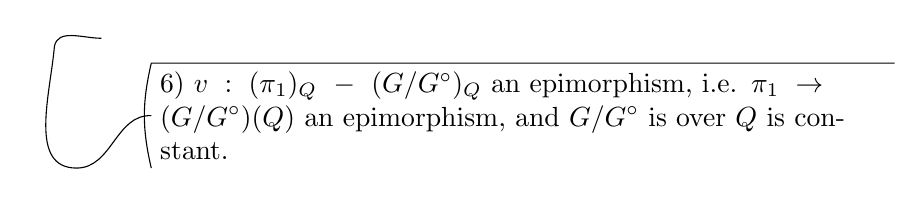
\begin{tikzpicture}
 \node[inner sep=3pt,text width=.76\linewidth,align=left] (addsix)
 {\inserted{6) $v:(\pi_1)_{\mathbb Q}\mathrel{-}(G/G^\circ)_{\mathbb Q}$ an epimorphism, i.e. $\pi_1\to(G/G^\circ)(\mathbb Q)$ an epimorphism, and $G/G^\circ$ \deleted{\unsure{is}} over $\mathbb Q$ is \uuline{constant}.}};
 \draw (addsix.north east) -- (addsix.north west) to[bend right=13] (addsix.south west);
 \draw (addsix.west) to[out=178,in=0] ([xshift=-27pt]addsix.south west) to[out=180,in=-95] ([xshift=-35pt,yshift=6pt]addsix.north west) to[out=80,in=180] ([xshift=-18pt,yshift=9pt]addsix.north west);
\end{tikzpicture}}

\deleted{\unsure{6|7}}7) For every closed point $s$ of $S$, the \unsure{Frobenius|Frobenius} element $f_s$ of $\pi_1(S,\xi)$ has \deleted{as image} \inserted{a} class in $G(A)$ \inserted{which corresponds to} the image of a conjugacy class of $G\deleted{\unsure{(A)|_{\mathbb Q}}}$ (recovers Weil \unsure{...|....}).

% slanted
\margin{will have to be \unsure{made precise|made precise} ...}

\deleted{\unsure{7|8}}8) $G_{\mathbb R}$ equipped with $i_1^{\mathbb C},i_2^{\mathbb C}$ of c) is a \uline{Hodge group}.

\deleted{\unsure{8|9}}9) (Modulo Tate) For every $\unsure{l|\ell}$, the image of $\pi_1\unsure{k|K|\xi}$ in $G(\mathbb Q_l)$ is a subgroup acting in a $\frac12$ simple way on every \deleted{\unsure{product|functor|generator}} $V\otimes_{\mathbb Q}\mathbb Q_l$ \deleted{\unsure{generates|generated} $\mathbb Q_l$ as}, (or \uline{one} such, with $\deleted{\unsure{V|D}}V$ \deleted{alone} faithful), and its algebraic envelope is $G_{\mathbb Q_l}$.

\deleted{\unsure{The composite} $\pi_1\to G(A)\to G(\mathbb Q_l)\unsure{\mathrel{-}|\to}G/G^\circ$}

% paper watermark, sideways
{\centering \textsc{\unsure{Extra} \unsure{Strong}}\\
\textit{\unsure{Ma}\unsure{in|nn}\unsure{ol|on}\unsure{uy|ny|y} \unsure{1808}}\par}
